\documentclass{standalone}
\usepackage{tikz}
\usetikzlibrary{positioning,shapes,shadows,arrows}

\begin{document}
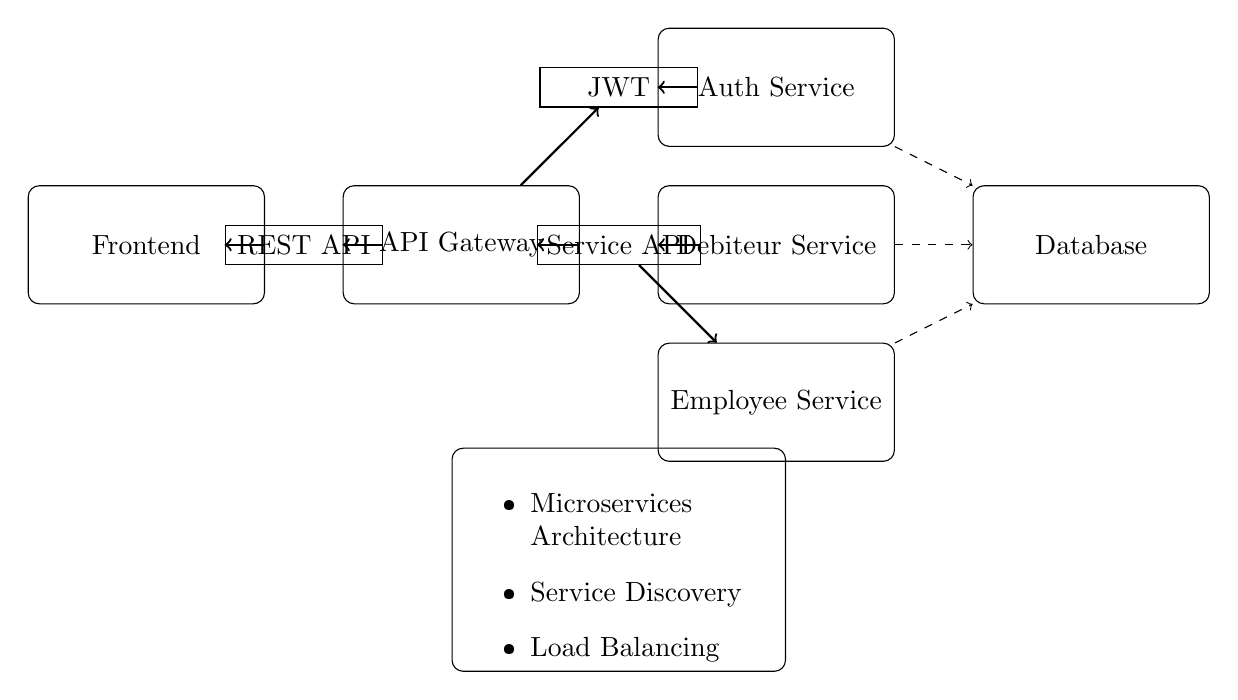
\begin{tikzpicture}[
    component/.style={draw, rectangle, rounded corners, minimum width=3cm, minimum height=1.5cm},
    interface/.style={draw, rectangle, minimum width=2cm, minimum height=0.5cm},
    arrow/.style={->, thick},
    dependency/.style={->, dashed}
]

% Components
\node[component] (frontend) at (0,0) {Frontend};
\node[component] (api) at (4,0) {API Gateway};
\node[component] (auth) at (8,2) {Auth Service};
\node[component] (debiteur) at (8,0) {Debiteur Service};
\node[component] (employee) at (8,-2) {Employee Service};
\node[component] (db) at (12,0) {Database};

% Interfaces
\node[interface] (frontend_api) at (2,0) {REST API};
\node[interface] (auth_api) at (6,2) {JWT};
\node[interface] (service_api) at (6,0) {Service API};

% Connections
\draw[arrow] (frontend) -- (frontend_api);
\draw[arrow] (frontend_api) -- (api);
\draw[arrow] (api) -- (auth_api);
\draw[arrow] (api) -- (service_api);
\draw[arrow] (auth_api) -- (auth);
\draw[arrow] (service_api) -- (debiteur);
\draw[arrow] (service_api) -- (employee);
\draw[dependency] (debiteur) -- (db);
\draw[dependency] (employee) -- (db);
\draw[dependency] (auth) -- (db);

% Notes
\node[draw, rectangle, rounded corners, text width=4cm] at (6,-4) {
    \begin{itemize}
        \item Microservices Architecture
        \item Service Discovery
        \item Load Balancing
    \end{itemize}
};

\end{tikzpicture}
\end{document} 